\documentclass[9pt]{beamer}

\usepackage{amsmath}
\usepackage{amsfonts}
\usepackage{amssymb}
\usepackage{mathtools}
\usepackage{amsthm}
\usepackage{bbm}

% \usepackage{amsmath}
% \usepackage{amsfonts}
% \usepackage{amssymb}
% \usepackage{mathtools}
% \usepackage{amsthm}
% \usepackage{bbm}
% % \usepackage{algpseudocode}
% \usepackage{interval}

\newcommand*{\citeauthorfoot}[1]{\citeauthor{#1}\footfullcite{#1}} 


\def\[#1\]{\begin{align*}#1 \end{align*}}  % Can do newlines in \[ \] env

\renewcommand*{\Re}{\operatorname{Re}}
\renewcommand*{\Im}{\operatorname{Im}}
\newcommand*{\ff}{\mathbb{F}}
\newcommand*{\zz}{\mathbb{Z}}
\newcommand*{\qq}{\mathbb{Q}}
\newcommand*{\rr}{\mathbb{R}}
\newcommand*{\cc}{\mathbb{C}}

\newcommand*\diff{\mathop{}\!\mathrm{d}}
\newcommand*\Diff[1]{\mathop{}\!\mathrm{d^#1}}\newcommand*{\defeq}{\vcentcolon=}
% \newcommand*{\defeq}{\vcentcolon=}
\newcommand*{\eqdef}{=\vcentcolon}

\newcommand*{\indic}{\mathbbm{1}}
\newcommand*{\Prob}{\mathbb{P}}
\newcommand*{\EE}{\mathbb{E}}

\newcommand*{\property}{\mathcal{P}}

\newcommand*{\Id}{\operatorname*{Id}}

\newcommand*{\LL}{\mathcal{L}}
\newcommand*{\GG}{\mathcal{G}}
\newcommand*{\MM}{\mathcal{M}}

\newcommand*{\normal}{\mathcal{N}}

\newcommand*{\Xx}{\mathbf{x}}
\newcommand*{\Yy}{\mathbf{y}}
\newcommand*{\Zz}{\mathbf{z}}

\newcommand*{\lb}{\log_2}

\DeclarePairedDelimiter{\ceil}{\lceil}{\rceil}
\DeclarePairedDelimiter{\floor}{\lfloor}{\rfloor}
\DeclarePairedDelimiter{\setx}{\lbrace}{\rbrace}
\DeclarePairedDelimiterXPP{\set}[1]{}{\lbrace}{\rbrace}{}{
  \renewcommand\given{\nonscript\:\delimsize\colon\nonscript\:\mathopen{}} #1
}
\DeclarePairedDelimiter{\brackets}{[}{]}
\DeclarePairedDelimiterX{\paren}[1]{(}{)}{#1}
%\DeclarePairedDelimiterX{\paren}[1]{(}{)}{
%  \ifblank{#1}{\:\cdot\:}{#1}
%}
\DeclarePairedDelimiterX{\abs}[1]{\lvert}{\rvert}{
  \ifblank{#1}{\:\cdot\:}{#1}
}
\DeclarePairedDelimiterX{\inp}[2]{\langle}{\rangle}{
  \ifblank{#1}{\:\cdot\:}{#1}
  \mathop{}\mathclose{}
  \delimsize\vert
  \mathopen{}\mathop{}
  \ifblank{#2}{\:\cdot\:}{#2}
}
\DeclarePairedDelimiterX{\norm}[1]{\lVert}{\rVert}{
  \ifblank{#1}{\:\cdot\:}{#1}
}
\DeclarePairedDelimiterXPP{\dist}[3]{d_{#1}}{(}{)}{}{#2, #3}

\providecommand\given{}
\DeclarePairedDelimiterXPP{\xprob}[1]{\Prob}{[}{]}{}{
  \renewcommand\given{\nonscript\:\delimsize\vert\nonscript\:\mathopen{}} #1
}
\DeclarePairedDelimiterXPP{\yprob}[2]{\Prob_{#1}}{[}{]}{}{
  \renewcommand\given{\nonscript\:\delimsize\vert\nonscript\:\mathopen{}} #2
}
\DeclarePairedDelimiterXPP{\uprob}[2]{\operatorname*{\Prob}_{\substack{#1}}}{[}{]}{}{
  \renewcommand\given{\nonscript\:\delimsize\vert\nonscript\:\mathopen{}} #2
}
\DeclarePairedDelimiterXPP{\xe}[1]{\EE}{[}{]}{}{#1}
\DeclarePairedDelimiterXPP{\xv}[1]{\mathbb{V}\mathrm{ar}}{[}{]}{}{#1}
\DeclarePairedDelimiterXPP{\xvar}[1]{\mathrm{Var}}{[}{]}{}{#1}

\DeclarePairedDelimiterXPP{\ye}[2]{\EE_{#1}}{[}{]}{}{#2}
\DeclarePairedDelimiterXPP{\ue}[2]{\operatorname*{\EE}_{\substack{#1}}}{[}{]}{}{#2}
\DeclarePairedDelimiterXPP{\xI}[1]{\indic}{[}{]}{}{#1}
\DeclarePairedDelimiterXPP{\yI}[2]{\indic_{#1}}{[}{]}{}{#2}



\newcommand*{\itern}{\brackets{n}}
\DeclarePairedDelimiter{\dual}{\bigl(}{\bigr)'}

\DeclarePairedDelimiterXPP{\xLn}[1]{\operatorname{\mathrm{ln}}}{(}{)}{}{#1}
%\DeclarePairedDelimiterXPP{\deg}[1]{\operatorname{\mathrm{deg}}}{(}{)}{}{#1}
\DeclarePairedDelimiterXPP{\Dim}[1]{\operatorname{\mathrm{dim}}}{(}{)}{}{#1}
\DeclarePairedDelimiterXPP{\Sp}[1]{\operatorname{\mathrm{Sp}}}{(}{)}{}{#1}
\DeclarePairedDelimiterXPP{\Ker}[1]{\operatorname{\mathrm{Ker}}}{(}{)}{}{#1}


\DeclarePairedDelimiterXPP{\fw}[2]{\mathbf{W}^{#1}}{[}{]}{}{#2}

\DeclarePairedDelimiterXPP{\Stab}[2]{\mathbf{Stab}_{#1}}{[}{]}{}{#2}
\DeclarePairedDelimiterXPP{\Spec}[2]{\mathbf{Spec}_{#1}}{[}{]}{}{#2}


% \newcommand*{\Ftwo}{\set{\pm 1}}


\newcommand*{\inftoinf}{\brackets{-\infty .. \infty}}
\newcommand*{\ivdlm}{,}

% \newcommand*{\holder}{H\"{o}lder }
% \newcommand*{\hct}{\(\paren[]{p, q, \rho}\)}

% obsolete
%\DeclarePairedDelimiterXPP{\xProb}[1]{\Prob}{[}{]}{}{#1}
%\DeclarePairedDelimiter{\abs}{\lvert}{\rvert}
%\DeclarePairedDelimiter{\norm}{\lVert}{\rVert}
%\DeclarePairedDelimiter{\set}{\lbrace}{\rbrace}
%\DeclarePairedDelimiterX{\zE}[1]{\operatorname*{\E}_{\substack{#1}}}{}{}
%\DeclarePairedDelimiter{\fw}{[}{]}



% Mooiere lege verzameling
\let\oldemptyset\emptyset
\let\emptyset\varnothing
% \let\oldphi\phi
% \let\phi\varphi


\usetheme[progressbar=frametitle]{metropolis}
% \usepackage[progressbar=frametitle]{sty/beamerthememetropolis}
\usepackage{appendixnumberbeamer}

\usepackage{booktabs}
% \usepackage[scale=2]{ccicons}

% \usepackage{pgfplots}% \usepgfplotslibrary{dateplot}

\usepackage{xspace}

\usepackage{color,soul}

\usepackage{caption}
% \usepackage{pgffor}

\usepackage{csquotes}
\usepackage{ragged2e}
\usepackage[
    % style=numeric,
    % citestyle=authoryear-icomp,
    backend=biber,
    maxbibnames=99,
]{biblatex}
\addbibresource{refs.bib}
\setbeamertemplate{bibliography item}{\insertbiblabel}

\usepackage{hyperref}


% \DeclarePairedDelimiter\floor{\lfloor}{\rfloor}

\metroset{block=fill}


% Authors and title
\newcommand*{\xauthor}{Ismani Nieuweboer}
\newcommand*{\xauthortiny}{I. Nieuweboer}
\newcommand*{\xtitle}{Wealth distribution models\xspace}
\newcommand*{\xsubtitle}{Duality and stationary distributions\xspace}
% \newcommand*{\xsubtitle}{\xspace}



\title{\xtitle}
\subtitle{\xsubtitle}
\date{2019-01-23}
% \date{}
\author{\xauthor}
\institute{University of Amsterdam}
% \titlegraphic{\hfill\includegraphics[height=1.5cm]{uvalogoofzo.pdf}}
% \setbeamertemplate{frame footer}{\xtitle -- \xauthortiny}
% \setbeamercolor{frame footer}{bg=beamer@blendedblue}

\begin{document}

\maketitle

% \begin{frame}{Table of contents}
%   \setbeamertemplate{section in toc}[sections numbered]
%   \tableofcontents[hideallsubsections]
% \end{frame}

% \section{Introduction}

\begin{frame}{}

\begin{figure}
    \centering
    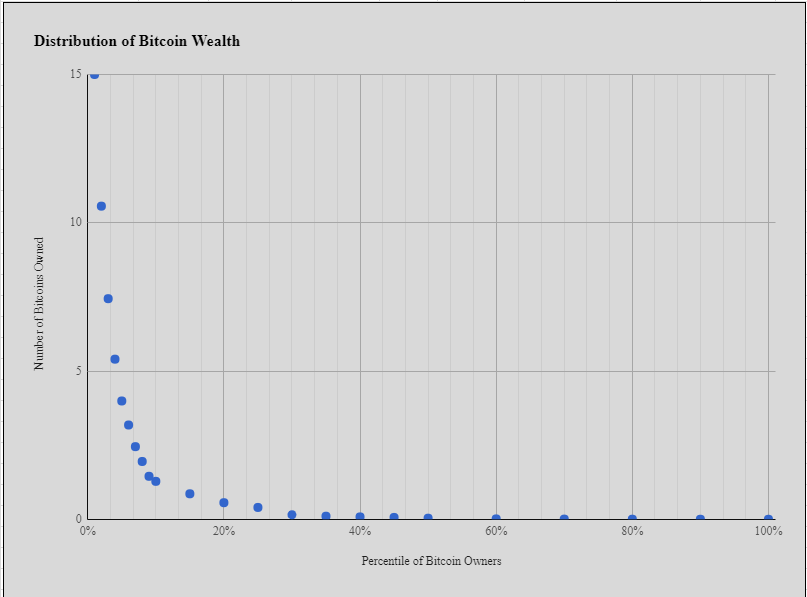
\includegraphics[width=0.9\textwidth]{bitcoin}
    % \caption{Caption}
    % \label{fig:my_label}
    
    \url{https://web.archive.org/web/20180501165520/https://arewedecentralizedyet.com/}
\end{figure}
    
\end{frame}

\begin{frame}{Introduction}
    \begin{itemize}
    \item Econophysics is a research field applying methods and ideas of statistical physics to economics
    \item Interest for economics from people originating from mathematics and physics is not new; for example Daniel Bernoulli, Jan Tinbergen -- see also \authorfootcite{yakovenko2009colloquium} for more examples
    \item This presentation will focus on concepts and results from \authorfootcite{cirillo2014duality}
    \end{itemize}
\end{frame}



\begin{frame}{Mathematical models and scientific method}
\begin{itemize}
    \item Model is mathematical
    \item Need to take care with interpretations and drawing conclusions about the real world -- empirical research is needed for this
    \item Need to take care especially due to the evident link between politics and economics
    % \item Also need to take care about language one uses -- one may still end up unconsciously make light political statements (?)
    % \item Hereby a warning to the listener to make sure the speaker does not cross these boundaries
\end{itemize}
\end{frame}


\begin{frame}{Concepts}
\begin{itemize}
    \item Money: Medium of exchange, store of value, unit of account (including debt)
    \item Wealth: Total of assets measured in monetary value
    \item Income: sum of all earnings over given period of time
    % \item Propensity to save:
    \item Agent: An entity which makes decisions given some model economy. In our case agent behavior is not studied and so no assumptions are made.
\end{itemize}
For example, one theoretical model in \authorcite{yakovenko2009colloquium} argues money is analogous to energy and income is analogous to power (energy per unit of time).
\end{frame}



\begin{frame}{Motivation and building block of model}
Suppose one starts with two agents with wealth $x$ and $y$. One can transfer wealth in one step in the following way for some $\epsilon \in [0, 1]$ (modelling some kind of transaction):
\[
% x' = \epsilon x + (1-\epsilon) y
% \\y' = (1-\epsilon) x + \epsilon y
x' &= \epsilon (x + y)
\\y' &= (1-\epsilon) (x + y)
\]
We have $x' + y' = x + y \eqdef s$, a conserved quantity, which occur in physics often (energy, momentum, etc).

Letting $T_{\epsilon}(x,y) = (x', y')$, we have a wealth-conserving map.
\pause
One can also consider that agents save a part of their wealth. For this let $\lambda \in [0, 1]$ be the \emph{saving propensity}. This naturally leads to
\[
T_{\lambda, \epsilon}(x,y)
= \lambda (x, y) + (1-\lambda) T_{\epsilon}(x,y)\]
which is still wealth-conserving.
\end{frame}



\begin{frame}{Motivation and building block of model}
\[
T_{\lambda, \epsilon}(x,y)
&= \lambda (x, y) + (1-\lambda) T_{\epsilon}(x,y)
\\&= \lambda (x, y) + (1-\lambda) (\epsilon (x + y), (1-\epsilon)(x + y))
\]

The paper refers to the case $\lambda=0$ as the \emph{energy} distribution model, and the case $\lambda \in (0, 1)$ as the \emph{wealth} distribution model.

We let $\epsilon \sim \nu(s, \cdot)$ be distributed along some probability measure.

\end{frame}



\begin{frame}{Process and generator}
The model is defined by a Markov process using the one-step redistribution in the same way as a continuous random walk (see lecture notes page 7). The state space is $[0, \infty)^2$ (no debt).

The process has to distribute wealth along the map $T_{\lambda, \epsilon}$ with $\epsilon \sim \nu(s, \cdot)$ with an $\operatorname*{Exp}(1)$ waiting time between each step.

For bounded continuous functions $f$ on this state space we hence let $L = P - I$ be the generator of the Markov process, with
\[
Pf(x, y) = \int_0^1 f(T_{\lambda, \epsilon}(x, y)) \nu(x+y, \diff \epsilon)
\]
\pause
i.e.
\[
Lf(x, y) = \int_0^1 \paren{f(T_{\lambda, \epsilon}(x, y)) - f(x, y) } \nu(x+y, \diff \epsilon).
\]
\end{frame}



\begin{frame}{Stationary and product measures}
Recall that a measure $\mu$ is a \emph{stationary} measure for the Markov process if and only if $\mu(Lf) = \int Lf \diff \mu = 0$.

% As the state space is $[0, \infty)^2$, we have that as a measure, $\mu\colon [0, \infty)^2 \to \rr_{\ge 0}$.
One can wonder whether the stationary measure behaves independently on $x$ and $y$, i.e. if we have $\mu(\diff x, \diff y) = \mu(x, y) \diff x \diff y = \mu(x) \mu(y) \diff x \diff y$ (abuse of notation -- function overloading as both measure and density)
\end{frame}



\begin{frame}{Research questions}
\begin{itemize}
\item What are the stationary distribution in this model?
\item Can we write the stationary distributions as a product?
\item Do there exist discrete dual processes (and if yes under which duality functions)?
\item Can anything be said for $N$ agents?
\end{itemize}
% not a physicist but model corresponds to physical model -- references given in paper
\end{frame}



\begin{frame}{Finding product distributions in case $\lambda = 0$}
\begin{itemize}
    \item For $\lambda = 0$, the measure $\mu$ is invariant if and only if $\nu(s, a) \propto \mu(as, (1-a)s)$.
    \item If $\mu$ is a product measure and $\nu$ does not depend on $s$, we have $\mu(x) \propto x^{b-1} \exp(-\lambda x)$ (Gamma distribution) and $\nu(s, \epsilon) = \nu(\epsilon) \propto \epsilon^{b-1}(1-\epsilon)^{b-1}$ (Beta distribution).
\end{itemize}
\end{frame}


\begin{frame}{Proofs}
% board
\end{frame}


\begin{frame}{Invariant measures in case $\lambda > 0$}
\begin{itemize}
    \item For $\lambda > 0$, the stationary measure can be characterized by the random variable
        \[
            \epsilon_{\infty}^{\lambda} = (1-\lambda)\sum_{k \ge 0} \lambda^k \epsilon_k
        \]
    \item All invariant measures have the same distribution as the random variable $(\epsilon_{\infty}^{\lambda}, 1 - \epsilon_{\infty}^{\lambda}) \cdot S$ where $S$ is a nonnegative random variable
    \item There are no product invariant measures in this case.
\end{itemize}
\end{frame}


\begin{frame}{Proofs}
\end{frame}


\begin{frame}{Duality -- a framework for our case}
The following is described in \authorcite{barbour2000transition}. Let $(X_t)_t$ be a Markov process with Markov generator $L$ on some continuous state space $\Omega$, with some invariant measure $\mu$.

Let $f_{\eta} \colon \Omega \to \Omega$ be nonnegative, for $\eta$ from a discrete state space $\Omega'$. Assume
\[
L f_{\eta} = \sum_{\zeta} r(\eta, \zeta) f_{\zeta}
\]
holds for rates $r$ with $r(\eta, \zeta) \ge 0$ if $\eta \ne \zeta$ and $r(\eta, \eta) \le 0$ for all $\eta$.
\pause
Then the following rates define a rate matrix $Q$ on $\Omega'$:
\[
q(\eta, \zeta) \defeq r(\eta, \zeta)\frac{\mu(f_{\zeta})}{\mu(f_{\eta})}. %board
\]
\pause
% Note that these indeed are rates as
% \[
% \sum_{\zeta} q(\eta, \zeta) = \frac{1}{\mu(f_{\eta})} \sum_{\zeta} r(\eta, \zeta)\mu(f_{\zeta}) = \frac{1}{\mu(f_{\eta})} \mu\paren*{\sum_{\zeta} r(\eta, \zeta) f_{\zeta}} = \frac{1}{\mu(f_{\eta})} \mu(L f_{\eta}) = 0.
% \]
and the associated Markov process  $(X_t')_t$ is dual to the original process with
\[
D(\eta, x) = \frac{f_{\eta}(x)}{\mu(f_{\eta})} % board
\]
% as
% \[
% LD(\eta, \cdot)(x)
% = \frac{f_{\eta}(x)}{\mu(f_{\eta})}
% = \sum_{\zeta} \frac{r(\eta, \zeta)}{\mu(f_{\eta})} f_{\zeta}(x)
% = \sum_{\zeta} \frac{q(\eta, \zeta)}{\mu(f_{\zeta})} f_{\zeta}(x)
% = \sum_{\zeta} q(\eta, \zeta) D(\zeta, x)
% = Q D(\cdot, x)(\eta)
% \]

% duality for generator implies duality for semigroup
which implies
% $\exp(tL) D(\eta, \cdot)(x) = \exp(tQ) D(\cdot, x)(\eta)$
\[
\ye{X}{D(\eta, X_t}
= \ye{\eta}{D(\eta_t, x}.
\]
\end{frame}


\begin{frame}{Duality for case $0 < \lambda < 1$}
Take $f_n(r) = r^n$. Then again taking generator
\[
Lf(r)
= \int_0^1 \paren{f(\lambda r + (1-\lambda) \epsilon) - f(r)} \nu(\diff \epsilon)
\]
we get
\[
Lf_n(r)
&= \int_0^1 (\lambda r + (1-\lambda) \epsilon)^n \nu(\diff \epsilon) - f_n(r)
\\&= \sum_{k=0}^n \lambda^k (1-\lambda)^{n-k} \int_0^1 \epsilon^{n-k} \nu(\diff \epsilon) f_k(r) - f_n(r)
= \sum_{k=0}^n r(n, k) f_k(r)
\]
and as $\nu_{\infty}^{\lambda}$ is the stationary measure, we get $q(k, n) = r(k, n) \frac{\nu_{\infty}^{\lambda}(f_k)}{\nu_{\infty}^{\lambda}(f_n)}$ as rates for the discrete dual process with duality function $D(n, r) = \frac{f_n(r)}{\nu_{\infty}^{\lambda}(f_n)}$.
\end{frame}



\begin{frame}{Diffusion process}
% The definition of a diffusion process is a Markov process for which the Kolmogorov forward equation is the Fokker--Planck equation.

% model of wealth distribution in microscopic time scales
In diffusion processes the idea is to consider very small time scales.

We consider the generator
\[
Af(x, y) = a(x, y)(\partial_x - \partial_y) + xy (\partial_x - \partial_y)^2
\]
Transforming with $s = x+y$ and $r = \frac{x}{s}$ gives
\pause
\[
Af(r)
= \frac{a(rs, (1-r)s)}{s}\partial_r + r(1-r) \partial_r^2
= \mu(r)\partial_r + h(r) \partial_r^2
\]
\end{frame}



\begin{frame}{Diffusion process}
\[
Af(r)
= \frac{a(rs, (1-r)s)}{s}\partial_r + r(1-r) \partial_r^2
= \mu(r)\partial_r + h(r) \partial_r^2
\]
The corresponding Fokker-Planck equation is
\pause
\[
\partial_t \psi(r) = 0 =
- \partial_r\brackets{\mu(r) \psi(r)} + \partial_r^2\brackets{h(r) \psi(r)}.
\]
from which we can derive the stationary measure
\pause
\[
\psi(r) \propto \frac{1}{r(1-r)}\exp\paren*{\int\frac{a(rs, (1-r)s)}{s} \diff r} % board
\]
Note: \authorcite{yakovenko2009colloquium} also mentions the Fokker--Planck equation in setting for income distributions.
%example linear case
\end{frame}




\begin{frame}{Result for $N$ agents}
% \begin{itemize}
%     \item
% \end{itemize}

Consider set of agents $\brackets{N} \defeq \set{1, 2, \hdots, N}$ and a symmetric random walk $\paren{\mathcal{X}_t}_t$ jumping at rate one according to transition probabilities $p(i,j)$, and (vector) process $x(t)$ of wealth of agents

\pause

Let $T_{\lambda, \epsilon}^{i, j}(x)$ for $x \in [0, \infty)^{\brackets{N}}$ such that
\[
T_{\lambda, \epsilon}^{i, j}(x)_k = T_{\lambda, \epsilon}(x_i, x_j)_k
% equal to \lambda x + (1- \lambda) \cdot (\epsilon OR 1-\epsilon) (x+y)
T_{\lambda, \epsilon}^{i, j}(x)_k = T_{\lambda, \epsilon}(x_i, x_j)_k
\]

\pause

The generator then is given by
\[
\mathcal{L}f(x) = \sum_{i, j} 2 p(i, j) \int \paren*{f(T_{\lambda, \epsilon}^{i, j}(x)) - f(x)} \nu(\sum_i x_i, \diff \epsilon)
\]

\pause

Result -- for $\mathbb{E}$ the expectation of the wealth process and $\mathcal{E}$ the expectation of the random walk process, we have
\[
\mathbb{E}_x\brackets{x_i(t)} = \mathcal{E}_i\brackets{x_{\mathcal{X}_{(1-\lambda)t}}}.
\]
\end{frame}




\begin{frame}{Link to statistical physics}
\begin{itemize}
    \item When $\nu(s, \diff \epsilon) = \diff\epsilon$ is uniform, the case $\lambda=0$ corresponds to the Kipnis-Marchioro-Presutti model (1982)
    \item When $\nu(s, \diff \epsilon) = \nu(\diff\epsilon)$ is Beta distributed, the case $\lambda=0$ corresponds to the thermalized Brownian energy process.
    % heat flow
\end{itemize}
% not a physicist
\end{frame}




\begin{frame}{Wrapping up}
  \begin{block}{Summary}
    \begin{itemize}
    \item A class of energy and wealth distribution models have been described
    \item With nonzero saving propensity these distributions do not have invariant measures
    \item The processes are dual to discrete processes and a class of associated diffusion processes exist
    \item A generalized model for $N$ agents is explored
    \end{itemize}
  \end{block}
  \begin{block}{Further reading}
    \begin{itemize}
    \item \authorcite{chakrabarti2013econophysics} has an overview of econophysical models of income and wealth distributions
    \item Further work building on paper discussed can be found through the citations: \url{https://scholar.google.com/scholar?cites=17345843713482550092}
    \end{itemize}
  \end{block}
  \pause
  \begin{center}
%   \vspace{1em}
  \huge{
  Thank you for your attention!
  }
  \end{center}
\end{frame}

\begin{frame}[allowframebreaks]{References}

%   \bibliography{ijcai17}
%   \bibliographystyle{abbrv}
  \printbibliography
\end{frame}

\end{document}
